
Most people, either knowingly or not, structure their software projects in an organized way. The organization is a positive side effect of methodologies and procedures such as object-oriented (OO) design, programming language rules, personal preference, habits, or dictated by project rules. While rules and conventions tend to be boring, adhering to them results in a more understandable project structure. As we can all agree, organized material is better for both human perception and computers. When procedure, rules, order, and organization exist, the computer can make sense of it. Documentation generation software leverages that fact to our benefit.

We will now introduce you to one of the most prominent documentation generation software for C and C++ programming languages: Doxygen. We will learn how we can integrate Doxygen with CMake to automatically generate documentation for CMake projects. 

Up next, the basics of Doxygen await.

\subsubsubsection{6.2.1\hspace{0.2cm}Understanding what Doxygen is}

Doxygen is a very popular documentation software for C++ projects that allows the generation of documentation from code. Doxygen understands C and C++ grammar and can see the code structure in a way that a compiler would see it. This allows Doxygen to dive into the structure of a software project and look into all class definitions, namespaces, anonymous functions, encapsulation, variables, inheritance relations, and so on. Doxygen combines this information with inline code documentation written by the programmer. The final result is human-readable documentation in various format that is compatible for both online and offline reading. 

But there is no such thing as a free lunch, as is the saying. In order to be able to make sense of code comments, Doxygen requires comments to be in a predefined set of formats. For the sake of not distracting from the focus of this chapter, please take a look at \url{https://www.doxygen.nl/manual/docblocks.html} to find out the comment formats compatible with Doxygen. We will be using Javadoc-style comments in our examples. An example Javadoc comment for a C++ function is provided here:

\begin{lstlisting}[style=styleCXX]
/**
* Does foo with @p bar and @p baz
*
* @param [in] bar Level of awesomeness
* @param [in] baz Reason of awesomeness
*/
void foo(int bar, const char* baz){}
\end{lstlisting}

Doxygen also requires a Doxyfile, which essentially contains all the parameters of documentation generation, such as output format, excluded file patterns, project name, and so on. Because of the sheer number of configuration parameters, configuring Doxygen may be intimidating at the start, but fear not—CMake will generate a Doxyfile for you too.

As we dive further into this chapter, you will start to see the benefits of using documentation generation software for your project. Through this, it is way easier to keep the documentation consistent with code, and the ability to read the code structure also makes graphing easier.

Enough theory for now. Let's begin using Doxygen together with CMake.

\subsubsubsection{6.2.2\hspace{0.2cm}Using Doxygen with CMake}

Make, being a C++-oriented build system generator, has good support for integrating external tools that are commonly used in C++ projects. As you would expect, integrating Doxygen with CMake is pretty straightforward. We'll utilize the FindDoxygen.cmake module of CMake to integrate Doxygen into our projects. This module is, by default, provided by the CMake installation and requires no extra setup.

FindDoxygen.cmake is, as the name suggests, a module package file designated to be consumed by the find\_package() CMake function. Its primary use is locating Doxygen in the environment, and also providing some extra utility functions to enable documentation generation in a CMake project. To illustrate Doxygen's abilities, we will be following the Chapter 6 - Example 01 example for this section. Our goal is to generate documentation for a simple calculator library along with its README file. The interface definition of this library looks like this:

\begin{lstlisting}[style=styleCXX]
class calculator : private calculator_interface {
public:
	/**
	* Calculate the sum of two numbers, @p augend lhs and
	@p addend
	*
	* @param [in] augend The number to which @p addend is
	added
	* @param [in] addend The number which is added to
	@p augend
	*
	* @return double Sum of two numbers, @p lhs and @p rhs
	*/
	virtual double sum(double augend, double addend)
	override;
	/**
	* Calculate the difference of @p rhs from @p lhs
	*
	* @param [in] minuend The number to which @p
	subtrahend is subtracted
	* @param [in] subtrahend The number which is to be
	subtracted from @p minuend
	*
	* @return double Difference of two numbers, @p minuend
	and @p subtrahend
	*/
	virtual double sub(double minuend, double subtrahend)
	override;
	/*...*/
}; // class calculator
\end{lstlisting}

The calculator class implements the class interface defined in the calculator\_interface class. It is properly documented in Javadoc format. We will expect Doxygen to generate application programming interface (API) documentation for the calculator and calculator\_interface classes, together with an inheritance diagram. The class definition is in the calculator.hpp file and can be found under the include/chapter6/ex01 subdirectory of the chapter6/ex01\_doxdocgen directory. Additionally, we have a Markdown file named README.md in the chapter6/ex01\_doxdocgen directory—this contains essential information about the example project's layout. We expect this file to be the main page of the documentation. As our input material is ready, let's start diving into the example further by inspecting the example's CMakeLists.txt file, chapter6/ex01\_doxdocgen/CMakeLists.txt, as usual. The CMakeLists.txt file begins with finding the Doxygen package, as can be seen here:

\begin{lstlisting}[style=styleCMake]
find_package(Doxygen)
set(DOXYGEN_OUTPUT_DIRECTORY"${CMAKE_CURRENT_BINARY_DIR}
	/docs")
set(DOXYGEN_GENERATE_HTML YES)
set(DOXYGEN_GENERATE_MAN YES)
set(DOXYGEN_MARKDOWN_SUPPORT YES)
set(DOXYGEN_AUTOLINK_SUPPORT YES)
set(DOXYGEN_HAVE_DOT YES)
set(DOXYGEN_COLLABORATION_GRAPH YES)
set(DOXYGEN_CLASS_GRAPH YES)
set(DOXYGEN_UML_LOOK YES)
set(DOXYGEN_DOT_UML_DETAILS YES)
set(DOXYGEN_DOT_WRAP_THRESHOLD 100)
set(DOXYGEN_CALL_GRAPH YES)
set(DOXYGEN_QUIET YES)
\end{lstlisting}

The find\_package(...) call will utilize the FindDoxygen.cmake module provided by the CMake installation to find Doxygen in the environment if present. The REQUIRED parameter is omitted in order to allow package maintainers to pack the project without having to install. This ensures that Doxygen in their environment is found before proceeding any further. The subsequent lines are setting several Doxygen configurations. These configurations will be placed into the Doxyfile that will be generated by CMake. Detailed descriptions for each option are listed here:

\begin{itemize}
\item 
DOXYGEN\_OUTPUT\_DIRECTORY: Sets the output directory for Doxygen.

\item 
DOXYGEN\_GENERATE\_HTML: Instructs Doxygen to emit HyperText Markup Language (HTML) output.

\item 
DOXYGEN\_GENERATE\_MAN: Instructs Doxygen to emit MAN page output.

\item 
DOXYGEN\_AUTOLINK\_SUPPORT: Allows Doxygen to automatically link language symbols and filenames to relevant documentation pages if available.

\item 
DOXYGEN\_HAVE\_DOT: Tells Doxygen the environment has the dot command available, which can be utilized for generating graphs. This will enable Doxygen to  enrich generated documentation with diagrams such as dependency, inheritance, and collaboration diagrams.

\item 
DOXYGEN\_COLLABORATION\_GRAPH: Tells Doxygen to generate collaboration diagrams for classes.

\item 
DOXYGEN\_CLASS\_GRAPH: Tells Doxygen to generate class diagrams for classes.

\item 
DOXYGEN\_UML\_LOOK: Instructs Doxygen to generate Unified Modeling Language (UML)-like diagrams.

\item 
DOXYGEN\_DOT\_UML\_DETAILS: Adds type and parameter information to UML diagrams

\item 
DOXYGEN\_DOT\_WRAP\_THRESHOLD: Sets the line wrapping threshold for UML diagrams.

\item 
DOXYGEN\_CALL\_GRAPH: Instructs Doxygen to generate call graphs for functions in function documentation.

\item 
DOXYGEN\_QUIET: Suppresses Doxygen output generated to standard output (stdout).
\end{itemize}

Doxygen's set of options is pretty extensive and offers a lot more than just the options we've covered. If you want to customize documentation generation further, take a look at the full list of parameters that can be used in Doxyfiles at \url{https://www.doxygen.nl/manual/config.html}. To set any Doxygen option in CMake, prefix the variable name with DOXYGEN\_ and set the desired value using set(). With that side note written down, let's go back to the example code. The CMake code shown before is followed by the target declarations. The following lines of code define a regular static library that contains our example code for the documentation:

\begin{lstlisting}[style=styleCMake]
add_library(ch6_ex01_doxdocgen_lib STATIC)
target_sources(ch6_ex01_doxdocgen_lib PRIVATE
	src/calculator.cpp)
target_include_directories(ch6_ex01_doxdocgen_lib PUBLIC
	include)
target_compile_features(ch6_ex01_doxdocgen_lib PRIVATE
	cxx_std_11)
\end{lstlisting}

Subsequently, the following lines of code define an executable that consumes the static library target defined before:

\begin{lstlisting}[style=styleCMake]
add_executable(ch6_ex01_doxdocgen_exe src/main.cpp)
target_compile_features(ch6_ex01_doxdocgen_exe PRIVATE
	cxx_std_11)
target_link_libraries(ch6_ex01_doxdocgen_exe PRIVATE
	ch6_ex01_doxdocgen_lib)
\end{lstlisting}

Lastly, the doxygen\_add\_docs(...) function is called to specify code that we wish to generate documentation from, as can be seen next:

\begin{lstlisting}[style=styleCMake]
doxygen_add_docs(
	ch6_ex01_doxdocgen_generate_docs
	"${CMAKE_CURRENT_LIST_DIR}"
	ALL
	COMMENT "Generating documentation for Chapter 6 - Example
		01 with Doxygen"
)
\end{lstlisting}
 
The doxygen\_add\_docs(...) function is a function provided by the FindDoxygen.cmake module. Its sole purpose is to provide a convenient way to create a CMake target for documentation generation without explicitly dealing with Doxygen. The signature for the doxygen\_add\_docs(...) function is shown here (non-relevant parameters are omitted):

\begin{lstlisting}[style=styleCMake]
doxygen_add_docs(targetName
	[filesOrDirs...]
	[ALL]
	[COMMENT comment])
\end{lstlisting}

The first parameter of the targetName function is the name for the documentation target. The function will generate a custom target named targetName. This target will trigger Doxygen and create documentation from the code when built. The next list of parameters, filesOrDirs, is a list of files or directories that contain the code we want to generate from the documentation. The ALL parameter is used to make CMake's ALL meta-target depend on the documentation target created by the doxygen\_add\_docs(...) function, so documentation generation is automatically triggered when the ALL meta-target is built. Lastly, the COMMENT parameter is for making CMake print a message to the output when the target is being built. COMMENT is primarily useful for diagnostic purposes so that we can quickly know whether documentation is being generated or not. 

After this brief introduction to doxygen\_add\_docs(...), let's go back to the example code and explain what the doxygen\_add\_docs(...) function call does in our scenario. It creates a target named ch6\_ex01\_doxdocgen\_generate\_docs, adds \$\{CMAKE\_CURRENT\_LIST\_DIR\} to the documentation generation directory, requests the ALL meta-target to depend on it, and specifies a COMMENT parameter that will be printed when the target is built.

All right—it's time to test whether this works or not. Go into the chapter\_6/ directory and configure the project in the build/ directory with the following command:

\begin{tcblisting}{commandshell={}}
cd chapter_6/
cmake –S . -B build/
\end{tcblisting}

Check the CMake output to see whether the configuration succeeded or not. If the configuration was successful, that means CMake succeeded to find Doxygen in the environment. You should be able to see that in the CMake output, as can be seen next:

\begin{tcblisting}{commandshell={}}
Found Doxygen: /usr/bin/doxygen (found version "1.9.1")
	found components: doxygen dot
\end{tcblisting}

After a successful configuration, let's try to build it with the following command:

\begin{tcblisting}{commandshell={}}
cmake --build build/
\end{tcblisting}

In the build output, you should be able to see that the text we've given into the COMMENT parameter is being printed to the CMake output. This means the documentation target is being built and Doxygen is running. Notice that we did not specify a -{}-target argument to the CMake build command, which effectively causes CMake to build the ALL meta-target. Since we have given the ALL argument to the doxygen\_add\_docs(...) function, a ch6\_ex01\_doxdocgen\_generate\_docs target is being built too. The output of the build command should look similar to the output given here:

\begin{tcblisting}{commandshell={}}
[ 20%] Generating documentation for Chapter 6 - Example 01
with Doxygen
Doxygen version used: 1.9.1
Searching for include files...
Searching for example files...
/*…*/
Running dot...
Running dot for graph 1/1
lookup cache used 9/65536 hits=13 misses=9
finished...
[ 20%] Built target ch6_ex01_doxdocgen_generate_docs
[ 40%] Building CXX object ex01_doxdocgen/CmakeFiles
  /ch6_ex01_doxdocgen_lib.dir/src/calculator.cpp.o
[ 60%] Linking CXX static library
libch6_ex01_doxdocgen_lib.a
[ 60%] Built target ch6_ex01_doxdocgen_lib
[ 80%] Building CXX object ex01_doxdocgen/CmakeFiles
  /ch6_ex01_doxdocgen_exe.dir/src/main.cpp.o
[100%] Linking CXX executable ch6_ex01_doxdocgen_exe
[100%] Built target ch6_ex01_doxdocgen_exe
\end{tcblisting}

It seems we have succeeded in building the project and the documentation. Let's inspect the generated documentation in the \$\{CMAKE\_CURRENT\_BINARY\_DIR\}/docs output folder, as follows:

\begin{tcblisting}{commandshell={}}
14:27 $ ls build/ex01_doxdocgen/docs/
html man
\end{tcblisting}

Here, we can see Doxygen has emitted the HTML and MAN page output into the html/ and man/ directories. Let's inspect the final result for each type. To inspect the generated MAN page, simply type the following:

\begin{lstlisting}[style=styleCMake]
man build/ex01_doxdocgen/docs/man/man3
	/chapter6_ex01_calculator.3
NAME
		chapter6::ex01::calculator - The 'calculator' class
		  interface.
SYNOPSIS
		#include <calculator.hpp>
	Static Public Member Functions
		static double sum (double augend, double addend)
		static double sub (double minuend, double
			subtrahend)
		static double mul (double multiplicand, double
			multiplier)
		static double div (double dividend, double divisor)
Detailed Description
		The 'calculator' class interface.
Member Function Documentation
	double chapter6::ex01::calculator::div (double
		dividend, double divisor) [static]
			Divide dividend with divisor
			Parameters
				dividend The number to be divided by divisor
				divisor The number by which divisor is to be
					divided
			Returns
				double Quotient of two numbers, dividend and
					divisor
Manual page chapter6_ex01_calculator.3 line 1 (press h for
	help or q to quit)
\end{lstlisting}

Great! Our code comments turned into a MAN page. Similarly, let's inspect the HTML output as well. Use a browser of your choice to open the build/ex01\_doxdocgen/docs/html/index.html file, as shown next:

\begin{tcblisting}{commandshell={}}
google-chrome build/ex01_doxdocgen/docs/html/index.html
\end{tcblisting}

This will display the main page of your documentation, as shown in the following screenshot:

\begin{center}
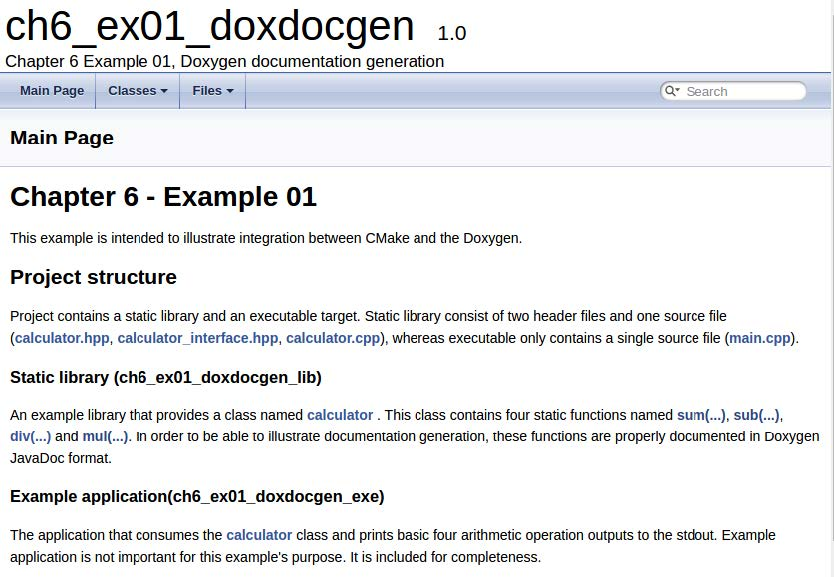
\includegraphics[width=1.\textwidth]{content/2/chapter6/images/1.jpg}\\
Figure 6.1 – The main page of the documentation
\end{center}

In the preceding screenshot, we can see that Doxygen has rendered the README.md Markdown file content into the main page. Note that the main page is just provided as an example. Doxygen can embed an arbitrary number of Markdown files into generated documentation. It even replaced filenames, class names, and function names with links to the relevant documentation. This is achieved by Doxygen's AUTOLINK feature and the @ref Doxygen command. Click on the calculator link under the Static library section of the main page to access API documentation for the calculator class. The calculator class documentation page should look similar to this:

\begin{center}
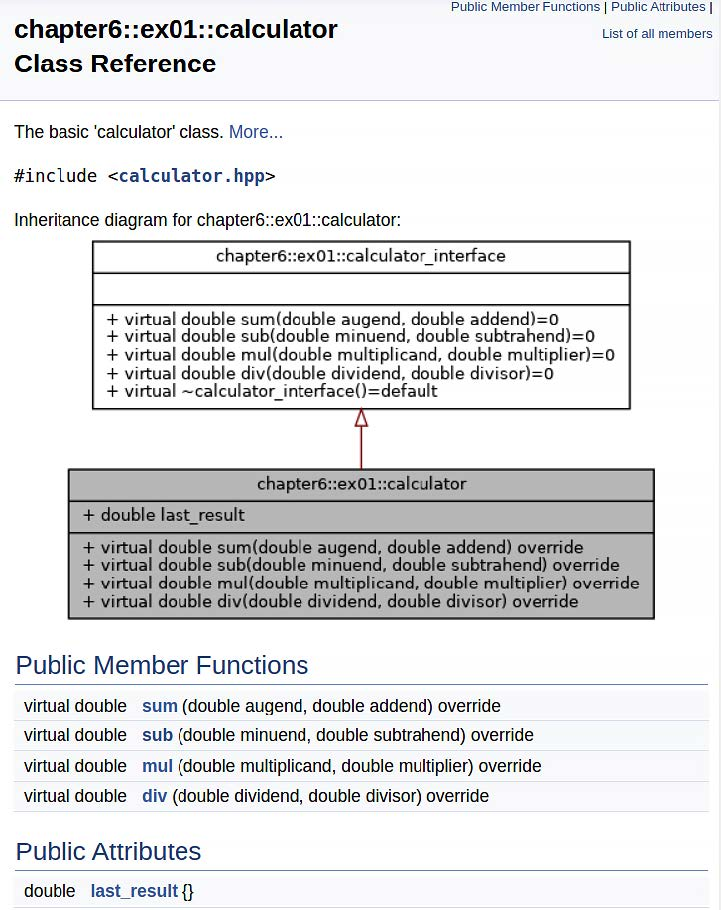
\includegraphics[width=1.\textwidth]{content/2/chapter6/images/2.jpg}\\
Figure 6.2 – Generated HTML documentation for the calculator class (basic layout)
\end{center}

In the preceding screenshot, we can see that Doxygen is aware that the calculator class inherits from calculator\_interface and draws an inheritance diagram for the calculator class.

\begin{tcolorbox}[colback=webgreen!5!white,colframe=webgreen!75!black,title=Note]
Doxygen requires the dot tool to render diagrams. dot is available in the Graphviz software package.
\end{tcolorbox}

Also, the generated diagrams contain function names and encapsulation symbols in UML style. Let's take a look at the detailed member function documentation shown in the following screenshot:

\begin{center}
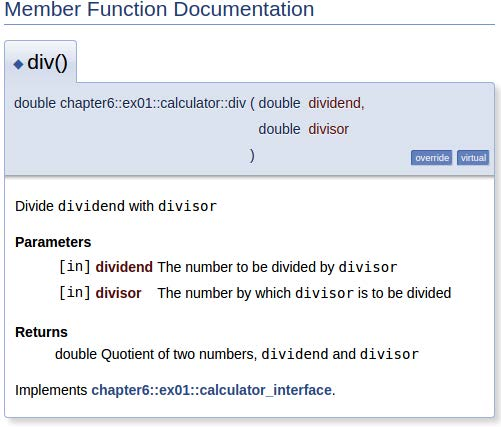
\includegraphics[width=1.\textwidth]{content/2/chapter6/images/3.jpg}\\
Figure 6.3 – Generated documentation for the div() function of the calculator class
\end{center}

As we can see in Figure 6.3, Doxygen did a pretty good job of putting the contents into a clear, readable layout. If you were reading this API documentation, you would be happy. Lastly, let's navigate to Files | File List | main.cpp to look into the documentation of main.cpp to illustrate what a dependency graph looks like. You can see a representation of the documentation page in the following screenshot:

\begin{center}
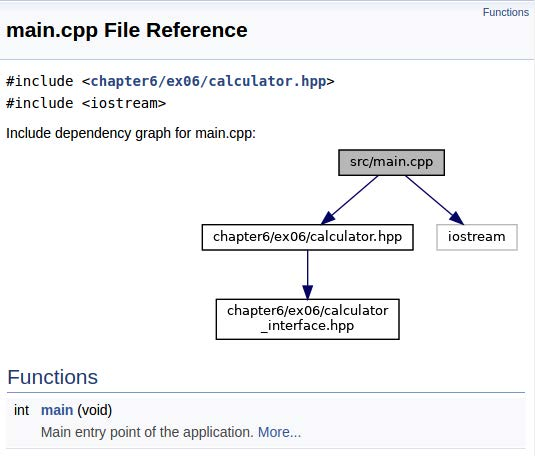
\includegraphics[width=1.\textwidth]{content/2/chapter6/images/4.jpg}\\
Figure 6.4 – main.cpp documentation page
\end{center}

The dependency graph in the preceding screenshot shows that the main.cpp file directly depends on iostream and chapter6/ex06/calculator.hpp and indirectly depends on chapter6/ex06/calculator\_interface.hpp files. It is pretty useful to have dependency information available in the documentation. The consumers will know exactly what the file dependencies are without having to dive into the code. If you scroll down a bit more, you will see a call graph for the main() function as well, as can be seen in the following screenshot:

\begin{center}
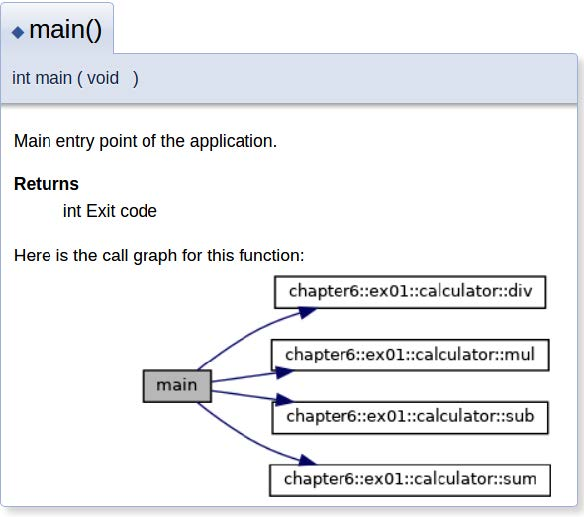
\includegraphics[width=0.8\textwidth]{content/2/chapter6/images/5.jpg}\\
Figure 6.5 – main() function call graph
\end{center}

Splendid! We have generated documentation with graphs for our code in two different formats with fewer than 20 lines of extra CMake code. How cool is that? Now, with that power in your hands, it is hard to find an excuse to avoid documentation. But our journey in this chapter is not over yet. The upcoming section will enrich our knowledge by teaching us how to embed custom UML diagrams into documentation. Let's go!
 
\subsubsubsection{6.2.3\hspace{0.2cm}Embedding custom UML diagrams into documentation}

In the previous section, we learned how to utilize Doxygen to generate diagrams and documentation for our CMake project, but not every diagram is inferable from the code. We might want to draw custom diagrams to illustrate the elaborate relationships of an entity with an external system that is not available in the code context. To tackle this, the obvious choice would be somehow making this context available in the code or comments to utilize documentation generation again. Well, as could be expected, this too is possible with Doxygen. Doxygen allows the embedding of PlantUML diagrams into comments, which will enable us to draw any diagram that PlantUML supports. But before starting to put PlantUML code in Doxygen comments, there's a small thing that must be taken care of: enabling PlantUML support in Doxygen. We have got ourselves a starting point. Let's roll!

Enabling PlantUML support in Doxygen is pretty easy. Doxygen requires a PLANTUML\_JAR\_PATH variable to be set to the location of the plantuml.jar file in the environment. So, we have to find out where that file is located. To do that, we will use the find\_path(...) CMake function. find\_path(...) is similar to find\_program(...), except it is designated for locating the path of files instead of program locations. So, that means we should be able to locate the path of plantuml.jar with find\_path(...), give this path to Doxygen, and ... profit! Let's put that theory to the test. We will be following Chapter 6 - Example 02 for this section. As ever, let's dive into the CMakeLists.txt file of the example code, located at the chapter\_6/ex02\_doxplantuml/CMakeLists.txt path. Let's start inspecting from the find\_path(...) call, as follows:

\begin{lstlisting}[style=styleCMake]
find_path(PLANTUML_JAR_PATH NAMES plantuml.jar HINTS
	"/usr/share/plantuml" REQUIRED)
find_package(Doxygen REQUIRED)
set(DOXYGEN_OUTPUT_DIRECTORY "${CMAKE_CURRENT_BINARY_DIR}
	/docs")
set(DOXYGEN_GENERATE_HTML YES)
set(DOXYGEN_AUTOLINK_SUPPORT YES)
set(DOXYGEN_PLANTUML_JAR_PATH "${PLANTUML_JAR_PATH}")
set(DOXYGEN_QUIET YES)
\end{lstlisting}

In the find\_path(...) call here, PLANTUML\_JAR\_PATH is the name of the output variable. NAMES is the filenames that will be searched in the search locations. HINTS is extra paths in addition to the default search locations. These are useful for discovering stuff in non-standard locations. Lastly, the REQUIRED parameter is used to make finding plantuml.jar a requirement, so CMake will fail and exit when plantuml.jar cannot be located. The following Doxygen configuration section is exactly the same as our previous example, Chapter 6 - Example 01, except we are setting DOXYGEN\_PLANTUML\_JAR\_PATH to the PlantUML directory path we found with the find\_path(...) call. Also, variables that are not required for this example are omitted too. Doxygen should be able to use PlantUML right now. Let's test that with an example PlantUML graph, embedded into the src/main.cpp source file, as follows:

\begin{lstlisting}[style=styleCXX]
/**
* @brief Main entry point of the application
  @startuml{system_interaction.png} "System Interaction
    Diagram"
  user -> executable : main()
  user -> stdin
  executable -> executable: read_stdin()
  executable -> stdout
  @enduml
* @return int Exit code
*/
int main(void) {
	std::cout << "Greetings from the echo application!" <<
	std::endl;
	std::string input;
	while (std::getline(std::cin, input)) {
		std::cout << input;
	}
}
\end{lstlisting}

The @startuml and @enduml Doxygen comment keywords are for indicating the beginning and the end of a PlantUML diagram, respectively. Regular PlantUML code can be placed inside of a @startuml - @enduml block. In our example, we have a simple system interaction diagram of the application. If everything goes as expected, we should see the embedded PlantUML diagram in the main() function's documentation. Let's generate documentation by building the example with the code shown here:
 
\begin{tcblisting}{commandshell={}}
cd chapter_6/
cmake -S ./ -B build/
cmake --build build/
\end{tcblisting}

The documentation for the second example should be built now. Open the generated build/ex02\_doxplantuml/docs/html/index.html HTML documentation with the browser of your choice, by running the following command:

\begin{tcblisting}{commandshell={}}
google-chrome build/ex02_doxplantuml/docs/html/index.html
\end{tcblisting}

This gives you the following output:

\begin{center}
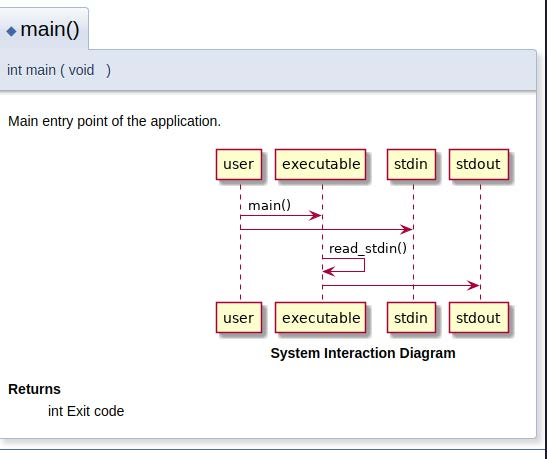
\includegraphics[width=0.8\textwidth]{content/2/chapter6/images/6.jpg}\\
Figure 6.6 – Embedded PlantUML diagram in the main() function documentation
\end{center}

In Figure 6.6, we can see that Doxygen has generated a PlantUML diagram and embedded it into the documentation. With that, we're now able to embed custom diagrams into our generated documentation as well. This will allow us to explain complicated systems and relationships without having to interact with external graphing tools.

Now, as we have the right tools for generating documentation, it's time to learn how to package and deliver them. In the next section, we will learn about ways of delivering documentation, together with the software involved.








